\documentclass[12pt]{report}
\usepackage{graphicx} % make it easy to load in images
\graphicspath{{./images/},{../../../plots/}} % where to find images
\usepackage[letterpaper, margin=1in]{geometry} % change margins 
\usepackage{fancyhdr} % add a header / footer 
\pagestyle{fancy}

\usepackage{amsmath}
\usepackage{amssymb}  
\usepackage{amsthm}
\usepackage{ulem} 

\usepackage{caption}  % for creating simple subfigures
\usepackage{subcaption}

\usepackage{titlesec} % redefine headings to remove "Chapter X"

\usepackage[labelfont=bf, textfont=md]{caption}

\usepackage{setspace}

\usepackage{hyperref}

\usepackage[color=cyan]{todonotes}

\usepackage[labelfont=bf]{caption}




\title{
	\large{Drunken Walking: A Novel Brownian Dynamics Simulation for the Mechanochemical Cycle of the Dynein Motor Protein}\vspace{1.5em}\\
	\normalsize{by}\\
	\large{John Waczak} \vspace{2em}\\ 
	\normalsize{an undergraduate thesis advised by David Roundy submitted to \\ 
		Department of Physics, Oregon State University}\vspace{2em}\\
	\normalsize{in partial fulfillment of the requirements for the degree of}\\
	\normalsize{Baccalaureate of Science in Physics}\vspace{1.5 em}\\
	\normalsize{Submitted \today}\vspace{3em}\\
	\includegraphics[width=0.5\columnwidth]{OSU_logo.png}\vspace{0.5em}\\
}
\date{}

\begin{document}
	\onehalfspacing
	
	\maketitle
	\chapter*{Abstract}
	\vspace{-3 em}word count: \textbf{282}\\
	
	The dynein molecule is a peculiar motor protein recognized for its odd stepping behavior. Sometimes it steps forwards. Other times it steps backwards. It has even been observed to occasionally shuffle by beginning a step with the same domain many times in row. These unique motions make dynein an interesting object of study, but its status as one of a select few minus-end directed motors makes understanding the mechanics of dynein’s motion vital to our understanding of the cell. When these motors misbehave, fundamental processes like axonal transport and muscle contraction fail. Experimental techniques for studying biomolecules have revealed much about the different conformational states achieved by dynein during its stepping cycle and have established a base of relevant statistics such step lengths, velocities, and generated forces among others. Despite these advancements, the ability to image the full molecule for an entire stepping cycle remains beyond current experimental capabilities. 
	
	To address this gap, we have developed a simplified, two-dimensional model for the dynein molecule. We treat the protein as a system of massive domains held together by rigid rods steered towards equilibrium configurations by spring like torques and time evolved using Brownian dynamics. With our current set of parameters, the model displays directed motion with step length and velocity distributions in agreement with experiment. Our simulations also suggest that there is no correlation between the conformation of dynein before and after it takes a step. Our results indicate that a more computationally efficient simulation can be achieved with a two state system where a post power stroke state is selected from a distribution via a Monte Carlo simulation and binding is then simulated with the full Brownian dynamics. 
	


	\tableofcontents
	\listoffigures
	%\listoftables
	
	
	\chapter{Introduction}
	\section{Cellular Processes}
	\subsection{The Cytoskeleton}
	\subsection{Mitosis} 
\section{Motor Proteins}
	\chapter{Dynein}
	\section{Directed Motion}
\section{Drunken Walking}
\section{Transporting Cargo}
\section{Experimental Stepping Statistics}
	\chapter{Theory}
	Having established some facts about motor proteins as well as specifics about dynein's many odd behaviors, we may begin our discussion of how to construct and test a physical model for its motion. First, we note that dynein's large cross section and mass (roughly 2 MDa) \cite{johnson1983structure} as compared to similar motor proteins such as Kinesin (a few hundred kDa) \cite{liao1998kinesin} amplifies the effect of interactions with the  aqueous environment of the cell. This results in a much more significant drag force as well as a random element from water molecule collisions that changes the overall dynamics of the system. The set of equations governing this motion is called Brownian dynamics and is what we use to simulate the trajectory of dynein along the microtubule. 
	\section{Brownian dynamics}
	To model dynein we treat its various domains (binding, motor, and tail) as spheres held together by massless rigid-rods. In general, the dynamics of a constant mass particle are governed by Newton's second law
	\begin{equation}
		\sum_i \mathbf{F}_i = \dot{\mathbf{p}} = m\ddot{\mathbf{x}}
	\end{equation}
	Thus, determining the dynamics of a system boils down to describing the various forces which act upon it and then solving the resulting differential equation for some set of initial conditions. For small particles in a solvent, there are three important forces to consider. The first is linear drag, which we write as 
	\begin{equation}
		F_\text{drag} = -\gamma\dot{\mathbf{x}}
	\end{equation}
	so that the drag force is proportional to the velocity by a factor $\gamma$. For a spherical particle of radius $a$ moving through a solvent with liquid viscosity $\eta$ this was derived by Stoke to be 
	\begin{equation}
		\gamma = 6\pi\eta a
	\end{equation}
	
	
	The second characteristic force of Brownian dynamics is a random force due to density fluctuations in the solvent which we denote $F_\text{rand}$. Finally, we might also consider how individual particles interact with each other through some interaction force. For us, this will be accomplished through the rigid rods that outline the structure of the protein by fixing the inter-domain distances via tension. Putting all of these forces together results in what is often called the \textit{Langevin Equation}.
	\begin{equation}
		 -\gamma\dot{\mathbf{x}}+\mathbf{F}_\text{rand} + \mathbf{F}_\text{interact} = m\ddot{\mathbf{x}} 
	\end{equation}
	
	If we assume further that $|\gamma\dot{\mathbf{x}}|\gg |m\ddot{\mathbf{x}}|$, or in other words, we take the limit of strong drag, then we arrive at the definition of Brownian Dynamics. This allows us to neglect the acceleration term resulting in the following differential equation
	\begin{equation}
		\dot{\mathbf{x}} = \frac{1}{\gamma}\left( \mathbf{F}_\text{interact} + \mathbf{F}_\text{rand} \right)
	\end{equation}
	which we must now solve for the equations of motion of our model. 
	
	
	\section{A Simplified Model for Dynein}
	As mentioned, we model dynein as a system of spherical domains held together by massless rigid-rods with the whole system moving according to Brownian dynamics. The random forces on each domain are responsible for diffusing the system and creating the expected chaotic motion, but in order to have dynein prefer walking towards one side of the microtubule, as is the case for real dynein, we need to impose some \textit{extra} structure on the protein. 
	
	\begin{figure}[hbt!]
		\centering
		\includegraphics[angle=-90, width=0.6\columnwidth]{torque_angles}
		\caption[One bound state]{Example of dynein in the one bound configuration with torque angles $\{\varphi_i\}$ shown.}
		\label{fig:torque angles}
	\end{figure}
	
	To do this we steer each domain towards an equilibrium configuration by a Hooke's law restorative torque with signed magnitude of the following form
	\begin{equation}
		\Gamma_i = -c_i\left(\varphi_i-\varphi_{i,\text{eq}}\right)
	\end{equation}
	Here the $c_i$ are spring constants (a free parameter of the model) and the set $\{\varphi_i\}$ are the angles measured between the $i-1$ and $i+1$ domains. Equally useful is the harmonic energy associated with each torque. These are given by
	\begin{equation}
		U_i = \frac{1}{2}c_i(\varphi_i-\varphi_{i,\text{eq}})^2
	\end{equation} 
	Bead-and-spring models such as this are common in molecular dynamics simulations as a way to model the interactions of the components of large molecules.\cite{bead-spring-model}. 
	
	
	Real dynein is composed of a pair of identical heavy chain legs. Therefore, our angle convention is chosen starting at the $0^{th}$ domain in figure \ref{fig:torque angles}. The same convention is then repeated for the second leg with the following correspondences as the two legs are identical. 
	\begin{align}
		\varphi_{0,eq} = \varphi_{4,eq} \\ 
		\varphi_{1,eq} = \varphi_{3,eq}
	\end{align}
	where the angles $\{\varphi_{i, \text{eq}}\}$ are the preferred angles of the system as illustrated in figure \ref{fig:torque angles}.\\
	
	 The torques on each domain are related to forces by 
	\begin{equation}
		\mathbf{\Gamma} = \mathbf{r}\times\mathbf{F}
	\end{equation}
	so that knowing the distance between each domains means that we have specified each of the $\mathbf{\Gamma}_i$ and $\mathbf{r}_i$. In order to dynamically move each domain, we must invert equation 3.10 to determine $\mathbf{F}_i$. However, there is no unique way to invert such a cross product. We must specify an algorithm for determining the forces that result from the torque on each domain. 
	
	\section{Calculating Forces and Torques}
	We would like our choice of forces to satisfy momentum conservation (linear and angular) as this condition is a physical requirement and serves to keep the energy of the structure in check across long simulations. Physically, this also imposes a requirement that no spring can move the entire molecule. To that end we must specify the spring forces for three cases: a motor domain, a tail domain, and an unbound binding domain. Having decided upon an algorithm for determining these forces, we can also calculate the force on a bound binding domain (attached to the microtubule) to estimate the maximum possible strain before unbinding occurs. This may prove interesting for future work but currently we do calculate these forces as a bound binding domain is static and therefore does not change its position while bound. \\ 
	
	To help us devise a reasonable method for applying the forces due to each torque, consider a small portion of dynein consisting of only three domains under the influence of \textbf{no} external forces. \\
	
	\begin{figure}[!hbt]
		\centering
		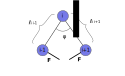
\includegraphics[angle =-90, width=0.475\columnwidth]{torque_forces.pdf}
		\caption[Torque related forces]{Toy model for three arbitrary domains. The force applied on each domain due to the torque on the $i^{th}$ domain is shown. Forces are chosen to be perpendicular the inter-domain separation and in the direction that would move $\varphi_i$ towards its equilibrium configuration. Equal and opposite forces are applied to the $i^{th}$.}
		\label{fig:torque_force}
	\end{figure}
	
	 Figure \ref{fig:torque_force} illustrates how the torque related forces on the $i^{th}$ domain and its two neighbors can be determined in this scenario. In general, equation (3.10) suggests we should pick the magnitude of the force on the $i^{th}$ domain due to the torque on the $j=i\pm1$ domains to be
	\begin{equation}
		F_{ij} \propto \Gamma_j / \ell_{ij}
	\end{equation}
	where $\ell_{ij}$ is the distance between the $i$ and $j$ domains. To make our lives easier, we can make the choice to apply the force perpendicular to the interdomain separation and in the direction of the equilibrium angle so that (3.11) is really an equality. If the $i^{th}$ domain were fixed in space, then we would be done. However, it is also free to move which means we should expect a force on it as well. We define the force on the $i^{th}$ domain to be the sum of the equal-and-opposite forces to the $i+1$ and $i-1$ domains. This results in the following properties
	\begin{equation}
		\sum\limits_{j=i-1}^{i+1}\mathbf{F}_j=0 \qquad\qquad \sum\limits_{j=i-1}^{i+1}\mathbf{\Gamma}_j = 0
	\end{equation}
	which indicate that the center of mass does not move (linear momentum conservation) and that angular momentum is conserved in the case of equal masses and equal distances (as desired). With this algorithm, we can loop through each domain and calculate the torque-related forces. For binding domains, there is only one neighboring domain to consider. 

	
	We are now armed with a way to calculate the forces on each domain due to the restorative torque. The only force which we are unable to calculate directly is the force due to tension. We will deal with this force via the method Lagrange multipliers as we solve for the equations of motion. 
	
	\section{Equations of Motion}
	The dynamics of each domain are determined by equation 3.5 so that in order to simulate the complicated structure we must solve a system of coupled first order differential equations. In doing so, it is convenient to introduce two states to distinguish between dynein's stepping and when both of its binding domains are attached to the microtubule. We shall refer to these configurations hereafter as the \textbf{one bound state} and the \textbf{both bound state} with the idea being that they directly correspond to the pre and post-stroke states defined by the mechanochemical cycle of \cite{cianfrocco2015mechanism}.  
	
	In the one bound state, all but one of the domains are free to diffuse while the last is attached to the microtubule. In the both bound state, both binding domains are attached. This slight difference in geometry between the two scenarios leads to two independent equations motion motion that require careful consideration when transitioning between states. The following sections detail the derivation of these equations of motion for each configuration. 
	
		\subsection{The one bound state}
		Figure \ref{fig:one bound} illustrates dynein in the one bound state with new angles $\{\theta_i\}$ chosen for convenience of calculation and computation.\\
		\begin{figure}[!hbt]
			\centering
			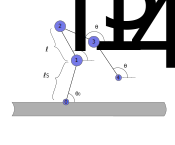
\includegraphics[angle=-90,width=0.8\columnwidth]{onebound}
			\caption[One bound angles]{The dynein model in the one bound state }
			\label{fig:one bound}  
		\end{figure}
		
		\noindent Here $\ell_S, \ell_T$ are fixed stalk and tail lengths. With some simple trigonometry, the positions of each domain are given by
		\begin{align}
		x's \quad &\begin{cases}
		x_0 = x_\text{bound} \\
		x_1 = x_0 + \ell_S \cos\theta_0 \\
		x_2 = x_1 + \ell_T \cos\theta_1 \\
		x_3 = x_2 + \ell_T \cos(\pi-\theta_3) = x_2 - \ell_T\cos\theta_3 \\
		x_4 = x_3 + \ell_S \cos(\pi-\theta_4) = x_3 - \ell_S\cos\theta_4
		\end{cases} &
		y's \quad &\begin{cases}
		y_0 = 0 \\
		y_1 = y_0 + \ell_S\sin\theta_0 \\
		y_2 = y_1 + \ell_T\sin\theta_1 \\
		y_3 = y_2 - \ell_T\sin\theta_3 \\
		y_4 = y_3 - \ell_S\sin\theta_4 
		\end{cases}
		\end{align} 
		
		\noindent Because equation (3.5) relates the forces on each domain to its velocity we need the time derivative of the above equations. 
		\begin{align}
		\dot{x}'s \quad \begin{cases}
		\dot{x}_0 = 0 \\
		\dot{x}_1 = \dot{x}_0-\ell_S\sin\theta_0 \dot{\theta}_0 \\
		\dot{x}_2 = \dot{x}_1-\ell_T\sin\theta_1 \dot{\theta}_1 \\
		\dot{x}_3 = \dot{x}_2+\ell_T\sin\theta_3 \dot{\theta}_3 \\
		\dot{x}_4 = \dot{x}_3+\ell_S\sin\theta_4 \dot{\theta}_4
		\end{cases} &
		\dot{y}'s \quad \begin{cases}
		\dot{y}_0 = 0 \\
		\dot{y}_1 = \dot{y}_0 + \ell_S\cos\theta_0\dot{\theta}_0 \\
		\dot{y}_2 = \dot{y}_1 + \ell_T\cos\theta_1\dot{\theta}_1 \\
		\dot{y}_3 = \dot{y}_2 - \ell_T\cos\theta_3\dot{\theta}_3 \\
		\dot{y}_4 = \dot{y}_3 - \ell_S\cos\theta_4\dot{\theta}_4
		\end{cases} 
		\end{align}
		
		The Brownian motion equation (3.5) also defines the velocity on each domain allowing us to write
		\begin{align}
			\dot{x}_i &= \frac{1}{\gamma_i}\Big(F_{i,\Gamma_i}^x+ \lambda_{i,i-1}(x_i-x_{i-1})+\lambda_{i,i+1}(x_i-x_{i+1})-F_{i,\text{rand}}^x\Big)\\
			\dot{y}_i &= \frac{1}{\gamma_i}\Big(F_{i,\Gamma_i}^y+ \lambda_{i,i-1}(y_i-y_{i-1})+\lambda_{i,i+1}(y_i-y_{i+1})-F_{i,\text{rand}}^y\Big) \notag
		\end{align}
		where superscript $x$ and $y$ denote the force components. 
		
		 At this point, comparing equations 3.13 with 3.14 reveals we have identified 8 nontrivial equations (x and y derivatives; ignoring bound binding domain 0). There are four unknown derivatives $\{\dot\theta_i\}$ and four unknown Lagrange multipliers $\{\lambda_{ij}\}$ which altogether form a linear system which we solve using Mathematica. For a detailed calculation see the appendices. 
		 
		 
		\subsection{The both bound state}
		For the both bound state, we no longer have a notion of bound and unbound domains. We therefore introduce a new notation, near and far, to identify each dimer. This is not purely for convenience of notation, but rather is important for storing data. We want the ability to calculate the total step length. Doing this requires knowledge of which motor domain initiates the stepping cycle. \\
		
		In the both bound state, both binding domains are attached to the microtubule and therefore, some degrees of freedom have been removed from our system. This enables us to simplify the dynamic equations in order to take advantage of the new, constrained geometry. To that end, we define a new coordinate system as shown in the following figure. 
		
		\begin{figure}[!hbt]
			\centering
			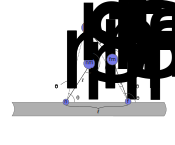
\includegraphics[width=0.75\columnwidth, angle=-90]{bothbound.pdf}
			\caption[The both bound state]{\textbf{Both bound} state with the new angles and lengths shown.}
			\label{fig:bothbound}
		\end{figure}
		
		Here, $\theta_{nm}$ and $\theta_{fm}$ can be obtained from the one bound state by 
		\begin{equation}
			\theta_{nm} = \theta_1+(\pi-\theta_0) \qquad \theta_{fm}= \theta_3 + (\pi-\theta_4) 
		\end{equation}
		Because the near and far binding domains are fixed, the only domains that we need to time evolve for the both bound state are the two motors (nm, fm) and the tail (T). Therefore, specifying $\theta_{nm}, \theta_{fm}$, and $\ell$ is enough to determine the geometry of the system. The intermediate variables are calculated by multiple applications of the law of cosines. 
		\begin{align}
			\ell_n &= \sqrt{\ell_s^2+\ell_T^2-2\ell_s\ell_T\cos(2\pi-\theta_{nm})} \\
			\ell_f &=  \sqrt{\ell_s^2+\ell_T^2-2\ell_s\ell_T\cos(2\pi-\theta_{fm})} \\
			\text{}\nonumber\\
			 \theta_n &= \arccos\left(\frac{\ell_n^2+\ell^2-\ell_f^2}{2\ell_n\ell}\right)\\
			\theta_f &= \pi-\arccos\left(\frac{\ell_f^2+\ell^2-\ell_n^2}{2\ell_f\ell}\right)\\
			\text{}\nonumber\\
			\theta_{n'} &= \arccos\left(\frac{\ell_n^2+\ell_s^2-\ell_t^2}{2\ell_n\ell_s}\right) \\
			\theta_{f'} &= \arccos\left(\frac{\ell_f^2+\ell_s^2-\ell_t^2}{2\ell_f\ell_s}\right) \\ 
			\text{}\nonumber \\ 
			\theta_{nb} &\equiv \theta_{n}-\theta_{n'} \\ 
			\theta_{fb} &\equiv \theta_{f}-\theta_{f'} 
		\end{align}
	   	with these angles and lengths defined, we can now easily define the positions 
	   		\begin{align}
	   	{x}'s \quad \begin{cases}
	   	{x}_{nm} = x_n+\ell_s\cos(\theta_{nb}) \\
	   	{x}_{fm} = x_f+\ell_s\cos(\theta_{fb}) \\
	   	{x}_{T} = x_{nm}+\ell_n\cos(\theta_n) 
	   	\end{cases} &
	   	{y}'s \quad \begin{cases}
	   	{y}_{nm} = \ell_s\sin(\theta_{nb}) \\
	   	{y}_{fm} = \ell_s\sin(\theta_{fb}) \\
	   	{y}_{t} = \ell_n\sin(\theta_n) 
	   	\end{cases} 
	   	\end{align}
		Now we have everything we need in order to repeat the process for the one bound state. Differentiating these equations will give us explicit formulas for the time derivative of the coordinates of each domain which we can then compare to the forces acting on each domain via the Brownian motion equation. Fortunately, the effort was well spent as we've reduced (3.14) to a system of six equation with 6 unknowns (one angle and one Lagrange multiplier for each \textit{moving} domain). 
		 
	\section{Binding and Unbinding}
	To keep the simulation simple, we have chosen an uncomplicated binding model which requires a minimum amount of assumptions. The two key processes, binding and unbinding, are controlled by two parameters called the binding rates (probability per unit time). For binding, we simply assume that a binding event occurs at a certain rate whenever a binding domain is close enough to the microtubule. That is, 
	
	\begin{equation}
	\begin{cases}
		\rho_{b} = k_b; & y_b < \varepsilon \\ 
		\rho_{b} = 0; & y_b > \varepsilon
	\end{cases}
	\end{equation}
	
	where $\rho_b$ is the rate and $k_b$ is a constant. \\
	
	Recently there has been evidence to show that dynein's step length depends on the tension applied at the linker between the two motor domains (e.g. the tail).\cite{cleary2014tension} This tension is high when the motor domains are far apart and small when they are together as illustrated in the following figure. \\
	\begin{figure}[!hbt]
		\centering
		\includegraphics[width=0.8\columnwidth]{yildiz_tension_dependence}
		\caption[Tension dependent stepping]{\textbf{Tension dependent stepping} is shown for a typical dynein (non-mutated). There is a clear, negative correlation between the step size and interhead separation. Data is clustered around trailing steps indicating that a higher tension leads to more stepping. Image taken from \cite{cleary2014tension}}
		\label{fig:yildiz_tension}
	\end{figure} 	
	As figure \ref{fig:yildiz_tension} indicates, a large interhead separation leads to more likely stepping. Furthermore, trailing steps are favored-- this means steps where the back foot begins the motion (like a normal human step) are more likely. To capture this behavior, we use an angle dependent exponential factor in the binding rate. That is 
	
	
	
	\begin{equation}
	\rho_{ub} = k_{ub}e^{c(\theta_b-\theta_{b,eq})}
	\end{equation}
	i.e. unbinding depends on the angular separation of the binding domain from it's equilibrium position. This means that for negative values of this constant, a large $\theta_b$ should yields a very small unbinding rate. Similarly, if $\theta_b$ is less than $\theta_{b,eq}$, then the unbinding rate is very large. This will favor the lagging foot because when dynein has a large interhead separation, the lagging $\theta_b$ is very small and the leading $\theta_b$ is very large as shown in the following figure. 
	
	\begin{figure}[!hbt]
		\centering
		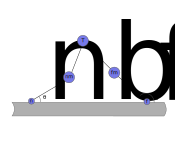
\includegraphics[width=0.7\columnwidth, angle=-90]{tension_dependence_edge_case}
		\caption[Stretched dynein]{\textbf{A Stretched dynein} illustrates the angular dependence of the unbinding model. In this configuration $\theta_{nb}$ is very small and is therefore much more likely to unbind than $\theta_{fb}$.}
	\end{figure}
	
	
	
	
	
	
	
	
	
	
	
	
	
	
	
	
	\chapter{Methods}
		
\section{The Code}
	\section{Time evolution: Euler's method}
	\subsection{The Random Force}
\section{Determining constants of the model}
The stalk and tail lengths $\ell_S, \ell_T$ as well as a set of equilibrium angles $\{\varphi_{i,\text{eq}}\}$ were determined by examining microscopy images of dynein in various configurations. 
\begin{figure}[hbt!]
	\centering
	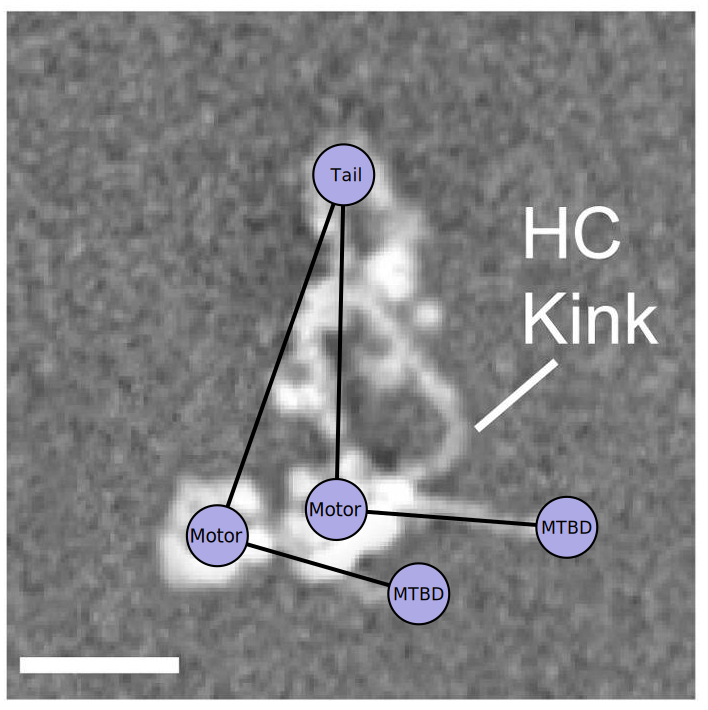
\includegraphics[width=0.3\columnwidth]{schematic-2-superimposed}
	\caption{Our model superimposed over microscopy image of Dynein \textbf{NOTE: add source} for determining lengths and equilibrium angles} 
	\label{fig:superimpmosed}
\end{figure}

\section{Testing the model} 
\subsection{Sanity Checks}
This sub section will be for the various methods we used to ensure our model is behaving reasonably 
\subsubsection{Verifying size of time step} 
Here I will talk about how we found autocorrelations functions for each domain energy at various values of dt in order to verify our time step is as large as can be
\subsubsection{Energy conservation and the Equipartion theorem} 
talk about code to check that we satisfy energy 
\subsection{Fitting to other studies} 	
	\chapter{Results \& Discussion}
	\todo[inline]{TODO: I plan to add description and section headings over break}
\todo[inline]{TODO: add discussion of powerstroke vs winch models. Discuss simple modifications to simulation parameters to try and fit for this alternate mechanochemical model}



	
\begin{figure}[!hbt]
	\centering
	\includegraphics[width=0.75\columnwidth]{paper_displacement_vs_step_length}
	\caption{\textbf{Two dimensional histogram} comparing the total signed step length to
			the signed initial displacement between the binding domains. A positive value
			indicates that the front foot made the step (leading). A negative value
			indicates the rear foot (lagging) made the step. Simulations show a strong,
			negative correlation. A similar fit from an experimental paper is plotted for comparison.}
\end{figure}
	
	
\begin{figure}[!hbt]
	\centering
	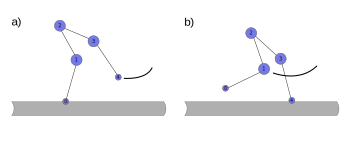
\includegraphics[angle=-90, width=1\columnwidth]{leading_vs_lagging}
	\caption{Diagram illustrating a leading foot step (a) and a lagging foot step (b).}
\end{figure}


\begin{figure}
	\centering
	\includegraphics[width=1\columnwidth]{paper_trajectory_plot}
	\caption{}
\end{figure}

	
\begin{figure}
	\centering
	\includegraphics[width=1\columnwidth]{paper_model_behavior}
	\caption{}
\end{figure}
\vspace{10em}

\todo[inline]{TODO: combine 5.1 with 5.2 to explain leading vs lagging}
\todo[inline]{TODO: consider removing leading lagging axis labels in 5.1 if redundant with figure caption} 
\todo[inline]{NOTE: it looks like there may be an issue with the middle most cartoon in 5.3. The tail does not appear to be the correct size}
\todo[inline]{TODO decrease overall width of tail in cartoon dynein. Increase thickness of stalk} 
\todo[inline]{TODO: Check to make sure time axis in final panel of fig 5.4 is actually a log scale} 
	\chapter{Conclusion}
	We have developed a Brownian dynamics simulation which effectively models the locomotion of the dynein motor protein. By manipulating our binding and unbinding rate parameters together with the spring constants for each domain, we are able to reproduce step length and velocity distributions as measured experimentally. Furthermore, directed motion towards the same end of the microtubule was achieved across all random number seeds without the need to introduce a separate model for the structure of the microtubule. 

In an effort to corroborate the results of research on the tension dependence of dynein stepping, we introduced an angle dependent unbinding rate which favors lagging foot steps at large inter-domain separations. Simulations with this unbinding model indicate that the one bound and both bound configurations are largely uncorrelated. In other words, the initial configuration of dynein does factor in to which domain steps, but it does not correlate with the final state after the next binding event. This unexpected result is contrary to experiment and has led us to begin developing a new simulation for which we only dynamically simulate the one bound state and use Monte Carlo methods to analyze distributions of possible both bound states. We anticipate that this new simulation will be significantly easier to implement and should lead to faster simulations. 


The flexible design and fast computation time relative to other simulation methods mean that our model can be easily applied to test other experimental hypotheses. For example, a popular mode of research is to use an optical tweezer to test how much force a dynein generates when pulling cargo. Our simulation can easily accommodate additional forces and will allow us to examine how the motion deviates from the case of a free dynein on a microtubule. Future work may also integrate a second dimension into the dynamics enabling us to simulate how dynein navigates around obstacles on it's 3 dimensional surface. By making small additions and adjustments like this, we believe that our simulation will help shed light on exactly how dynein moves throughout the cell. 
\bibliography{references}
\bibliographystyle{plain}
\end{document}
